%%%
%
% $Autor: Wings $
% $Datum: 2021-05-14 $
% $Pfad: GitLab/MLEdgeComputer $
% $Dateiname: LensCalibrationTool
% $Version: 4620 $
%
% !TeX spellcheck = de_DE/GB
%
%%%



\chapter{Lens Calibration Tool}


Arducam Lens Calibration Tool, Sichtfeld (Field of View, FoV) Test Chart Folding Card, Pack of 2

\url{https://www.amazon.com/-/de/dp/B0872Q1RLD/ref=sr_1_40?__mk_de_DE=ÅMÅŽÕÑ&dchild=1&keywords=arducam&qid=1622358908&sr=8-40}

\begin{description}
  \item[Multifunktional für Objektiv:] Objektivfokus kalibrieren, FoV messen und Schärfe abschätzen
  \item[Einfach zu bedienen:] Schnelle Einrichtung in Sekunden und Messung in Minuten mit Online-Videotutorial.
  \item[Ein handliches Werkzeug:] Einfaches Ermitteln des Sichtfelds des Objektivs ohne Berechnung
  \item[Sauber und aufgeräumt:] Faltbarer Kartenstil, mehrfach gefaltet und aufgerollt für schnelle Einstellung und bessere Lagerung
  \item[Anwendung:] Fokuskalibrierung, Schärfeschätzung und Bildfeld-Schnellmessung für M12, CS-Mount, C-Mount und DSLR-Objektive.

\end{description}
\url{https://www.arducam.com/product/arducam-lens-calibration-tool-field-of-view-fov-test-chart-folding-card-pack-of-2/}


\begin{figure}
  \begin{center}
    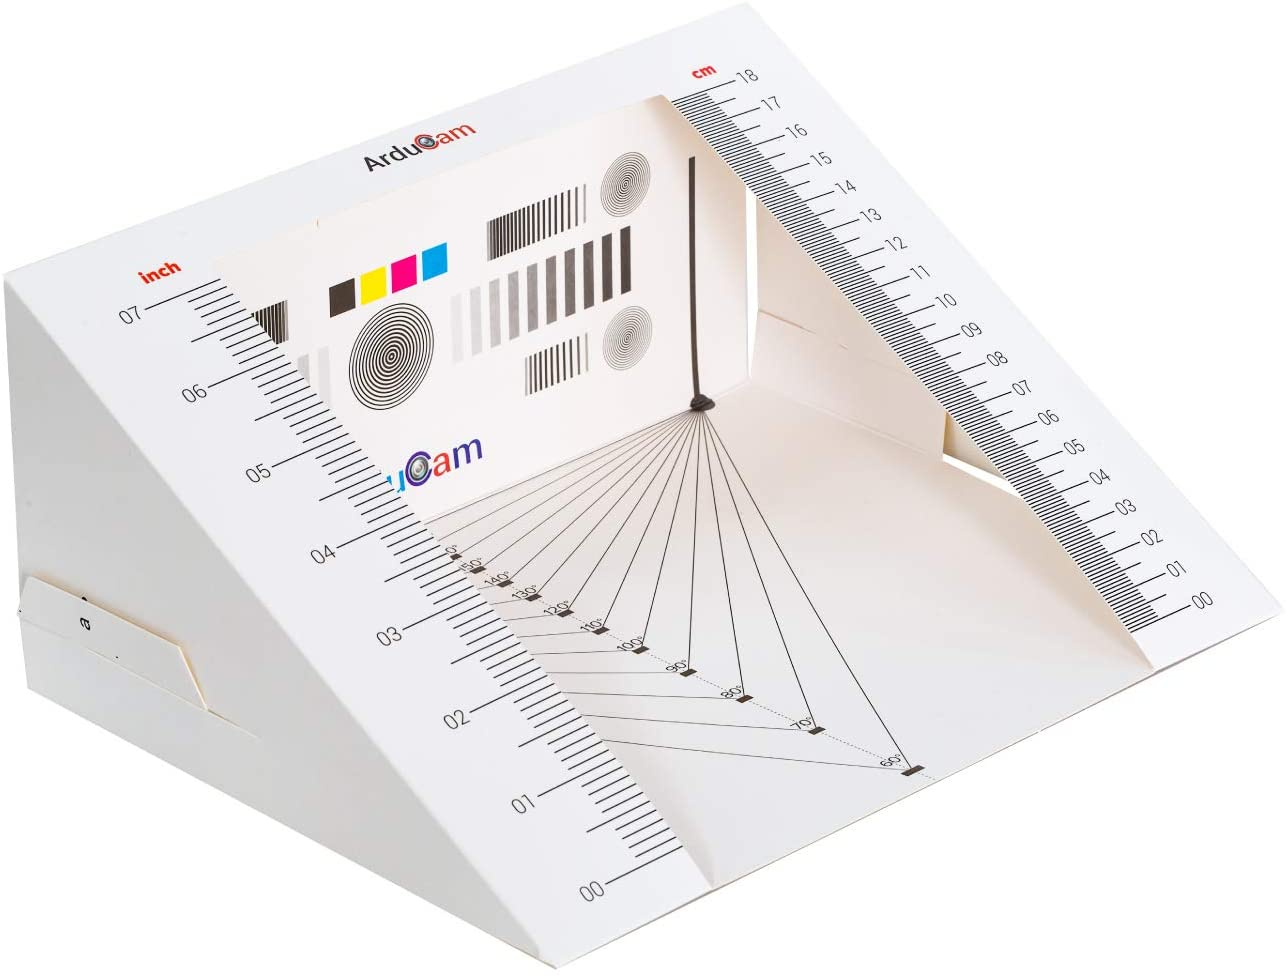
\includegraphics[scale=0.15]{CAM/LensCalibrationTool/LensCalibrationTool}
    \quad 
    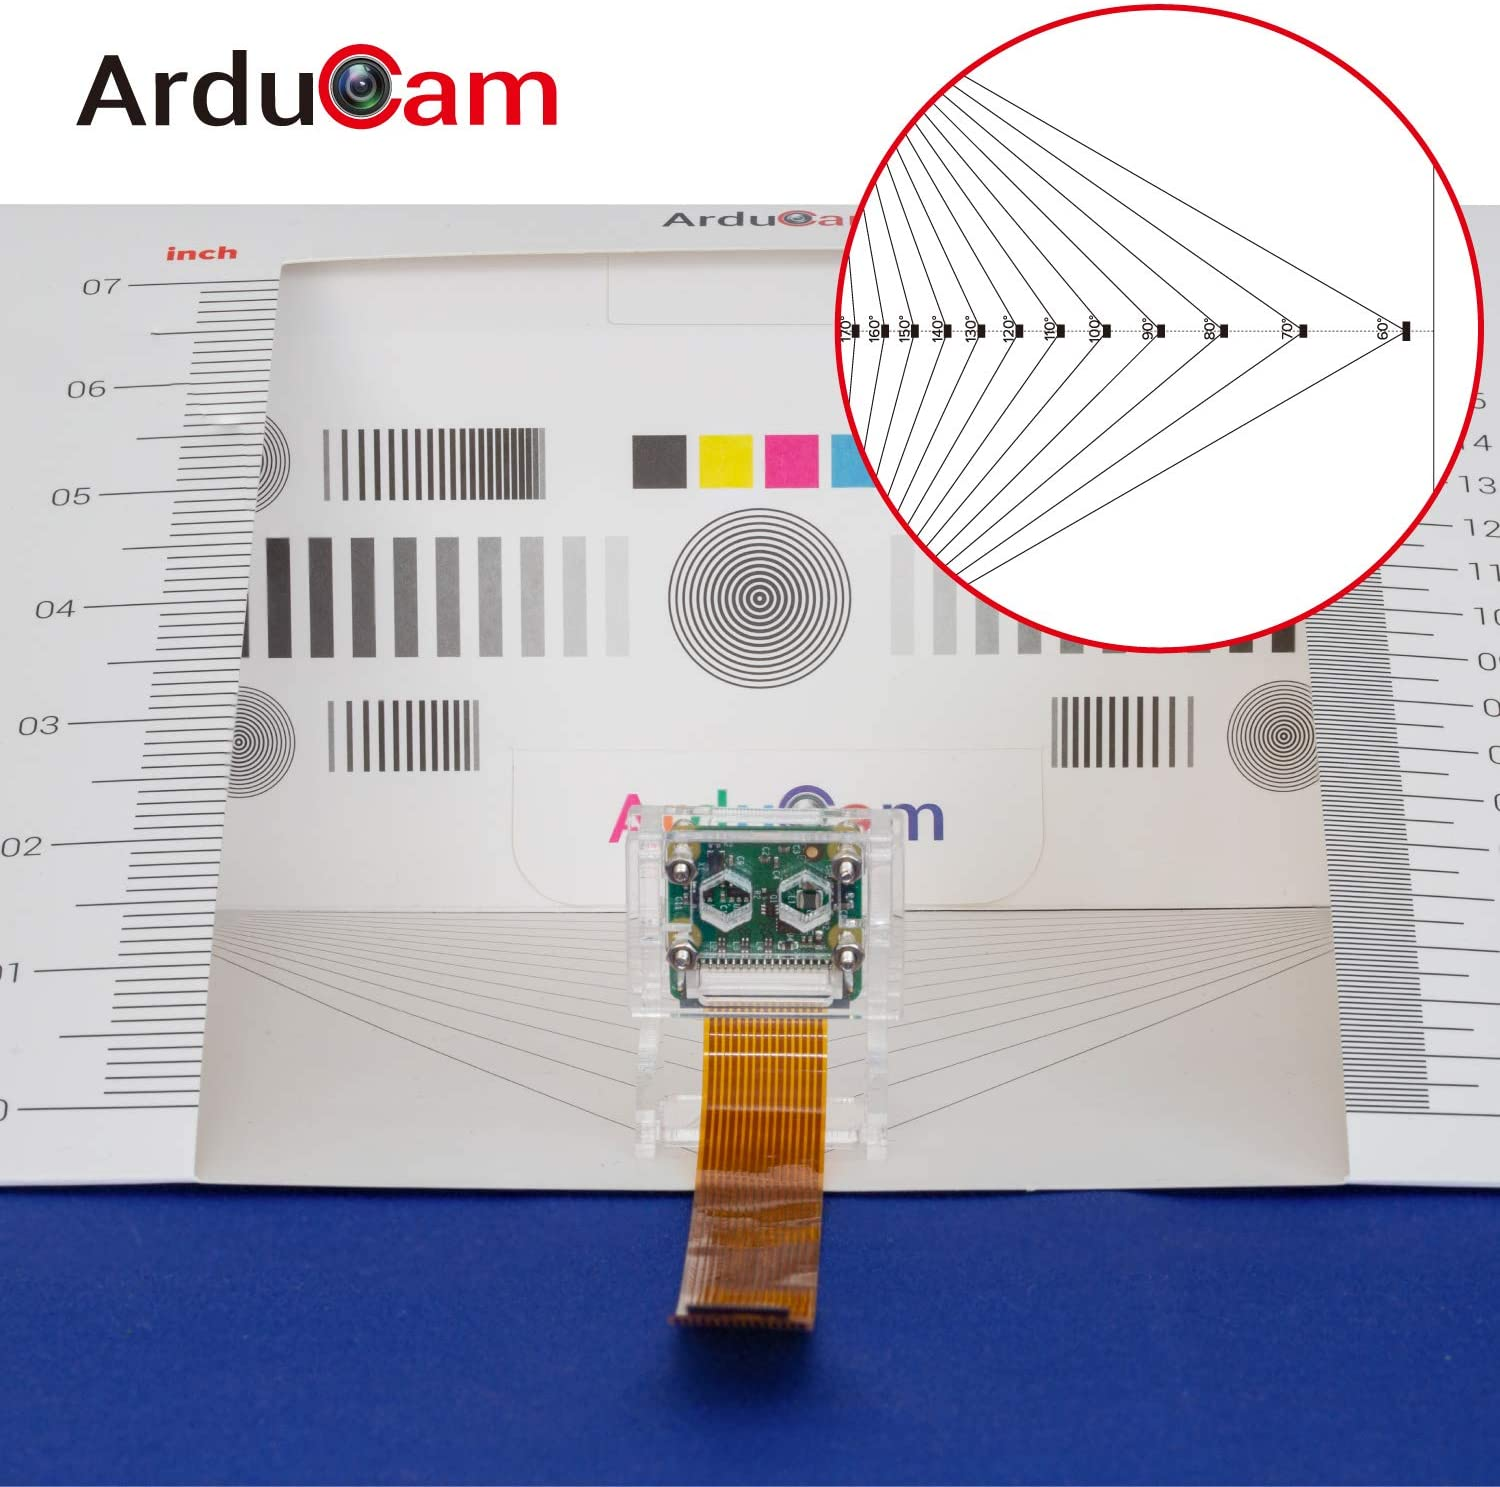
\includegraphics[scale=0.1]{CAM/LensCalibrationTool/LensCalibrationTool4}
  
    \caption{Kalibrierungswerkzeug der Firma Arducam; \cite{Arducam:2021}}
  \end{center}    
\end{figure}

\section{Übersicht}

Sind Sie immer noch frustriert von der Berechnung des FOV Ihrer Objektive und den unscharfen Bildern? Arducam hat jetzt ein multifunktionales Tool für Objektive veröffentlicht, mit dem Sie das Sichtfeld des Objektivs ohne Berechnung erhalten und den Objektivfokus schnell und einfach kalibrieren können.

\section{Applications}

Focus calibration, sharpness estimation and field of view quick measuring for M12, CS-Mount, C-Mount, and DSLR lenses

\section{Package Contents}

2*Foldable Lens Calibration Card

